\documentclass[1p]{elsarticle_modified}
%\bibliographystyle{elsarticle-num}

%\usepackage[colorlinks]{hyperref}
%\usepackage{abbrmath_seonhwa} %\Abb, \Ascr, \Acal ,\Abf, \Afrak
\usepackage{amsfonts}
\usepackage{amssymb}
\usepackage{amsmath}
\usepackage{amsthm}
\usepackage{scalefnt}
\usepackage{amsbsy}
\usepackage{kotex}
\usepackage{caption}
\usepackage{subfig}
\usepackage{color}
\usepackage{graphicx}
\usepackage{xcolor} %% white, black, red, green, blue, cyan, magenta, yellow
\usepackage{float}
\usepackage{setspace}
\usepackage{hyperref}

\usepackage{tikz}
\usetikzlibrary{arrows}

\usepackage{multirow}
\usepackage{array} % fixed length table
\usepackage{hhline}

%%%%%%%%%%%%%%%%%%%%%
\makeatletter
\renewcommand*\env@matrix[1][\arraystretch]{%
	\edef\arraystretch{#1}%
	\hskip -\arraycolsep
	\let\@ifnextchar\new@ifnextchar
	\array{*\c@MaxMatrixCols c}}
\makeatother %https://tex.stackexchange.com/questions/14071/how-can-i-increase-the-line-spacing-in-a-matrix
%%%%%%%%%%%%%%%

\usepackage[normalem]{ulem}

\newcommand{\msout}[1]{\ifmmode\text{\sout{\ensuremath{#1}}}\else\sout{#1}\fi}
%SOURCE: \msout is \stkout macro in https://tex.stackexchange.com/questions/20609/strikeout-in-math-mode

\newcommand{\cancel}[1]{
	\ifmmode
	{\color{red}\msout{#1}}
	\else
	{\color{red}\sout{#1}}
	\fi
}

\newcommand{\add}[1]{
	{\color{blue}\uwave{#1}}
}

\newcommand{\replace}[2]{
	\ifmmode
	{\color{red}\msout{#1}}{\color{blue}\uwave{#2}}
	\else
	{\color{red}\sout{#1}}{\color{blue}\uwave{#2}}
	\fi
}

\newcommand{\Sol}{\mathcal{S}} %segment
\newcommand{\D}{D} %diagram
\newcommand{\A}{\mathcal{A}} %arc


%%%%%%%%%%%%%%%%%%%%%%%%%%%%%5 test

\def\sl{\operatorname{\textup{SL}}(2,\Cbb)}
\def\psl{\operatorname{\textup{PSL}}(2,\Cbb)}
\def\quan{\mkern 1mu \triangleright \mkern 1mu}

\theoremstyle{definition}
\newtheorem{thm}{Theorem}[section]
\newtheorem{prop}[thm]{Proposition}
\newtheorem{lem}[thm]{Lemma}
\newtheorem{ques}[thm]{Question}
\newtheorem{cor}[thm]{Corollary}
\newtheorem{defn}[thm]{Definition}
\newtheorem{exam}[thm]{Example}
\newtheorem{rmk}[thm]{Remark}
\newtheorem{alg}[thm]{Algorithm}

\newcommand{\I}{\sqrt{-1}}
\begin{document}

%\begin{frontmatter}
%
%\title{Boundary parabolic representations of knots up to 8 crossings}
%
%%% Group authors per affiliation:
%\author{Yunhi Cho} 
%\address{Department of Mathematics, University of Seoul, Seoul, Korea}
%\ead{yhcho@uos.ac.kr}
%
%
%\author{Seonhwa Kim} %\fnref{s_kim}}
%\address{Center for Geometry and Physics, Institute for Basic Science, Pohang, 37673, Korea}
%\ead{ryeona17@ibs.re.kr}
%
%\author{Hyuk Kim}
%\address{Department of Mathematical Sciences, Seoul National University, Seoul 08826, Korea}
%\ead{hyukkim@snu.ac.kr}
%
%\author{Seokbeom Yoon}
%\address{Department of Mathematical Sciences, Seoul National University, Seoul, 08826,  Korea}
%\ead{sbyoon15@snu.ac.kr}
%
%\begin{abstract}
%We find all boundary parabolic representation of knots up to 8 crossings.
%
%\end{abstract}
%\begin{keyword}
%    \MSC[2010] 57M25 
%\end{keyword}
%
%\end{frontmatter}

%\linenumbers
%\tableofcontents
%
\newcommand\colored[1]{\textcolor{white}{\rule[-0.35ex]{0.8em}{1.4ex}}\kern-0.8em\color{red} #1}%
%\newcommand\colored[1]{\textcolor{white}{ #1}\kern-2.17ex	\textcolor{white}{ #1}\kern-1.81ex	\textcolor{white}{ #1}\kern-2.15ex\color{red}#1	}

{\Large $\underline{12a_{0386}~(K12a_{0386})}$}

\setlength{\tabcolsep}{10pt}
\renewcommand{\arraystretch}{1.6}
\vspace{1cm}\begin{tabular}{m{100pt}>{\centering\arraybackslash}m{274pt}}
\multirow{5}{120pt}{
	\centering
	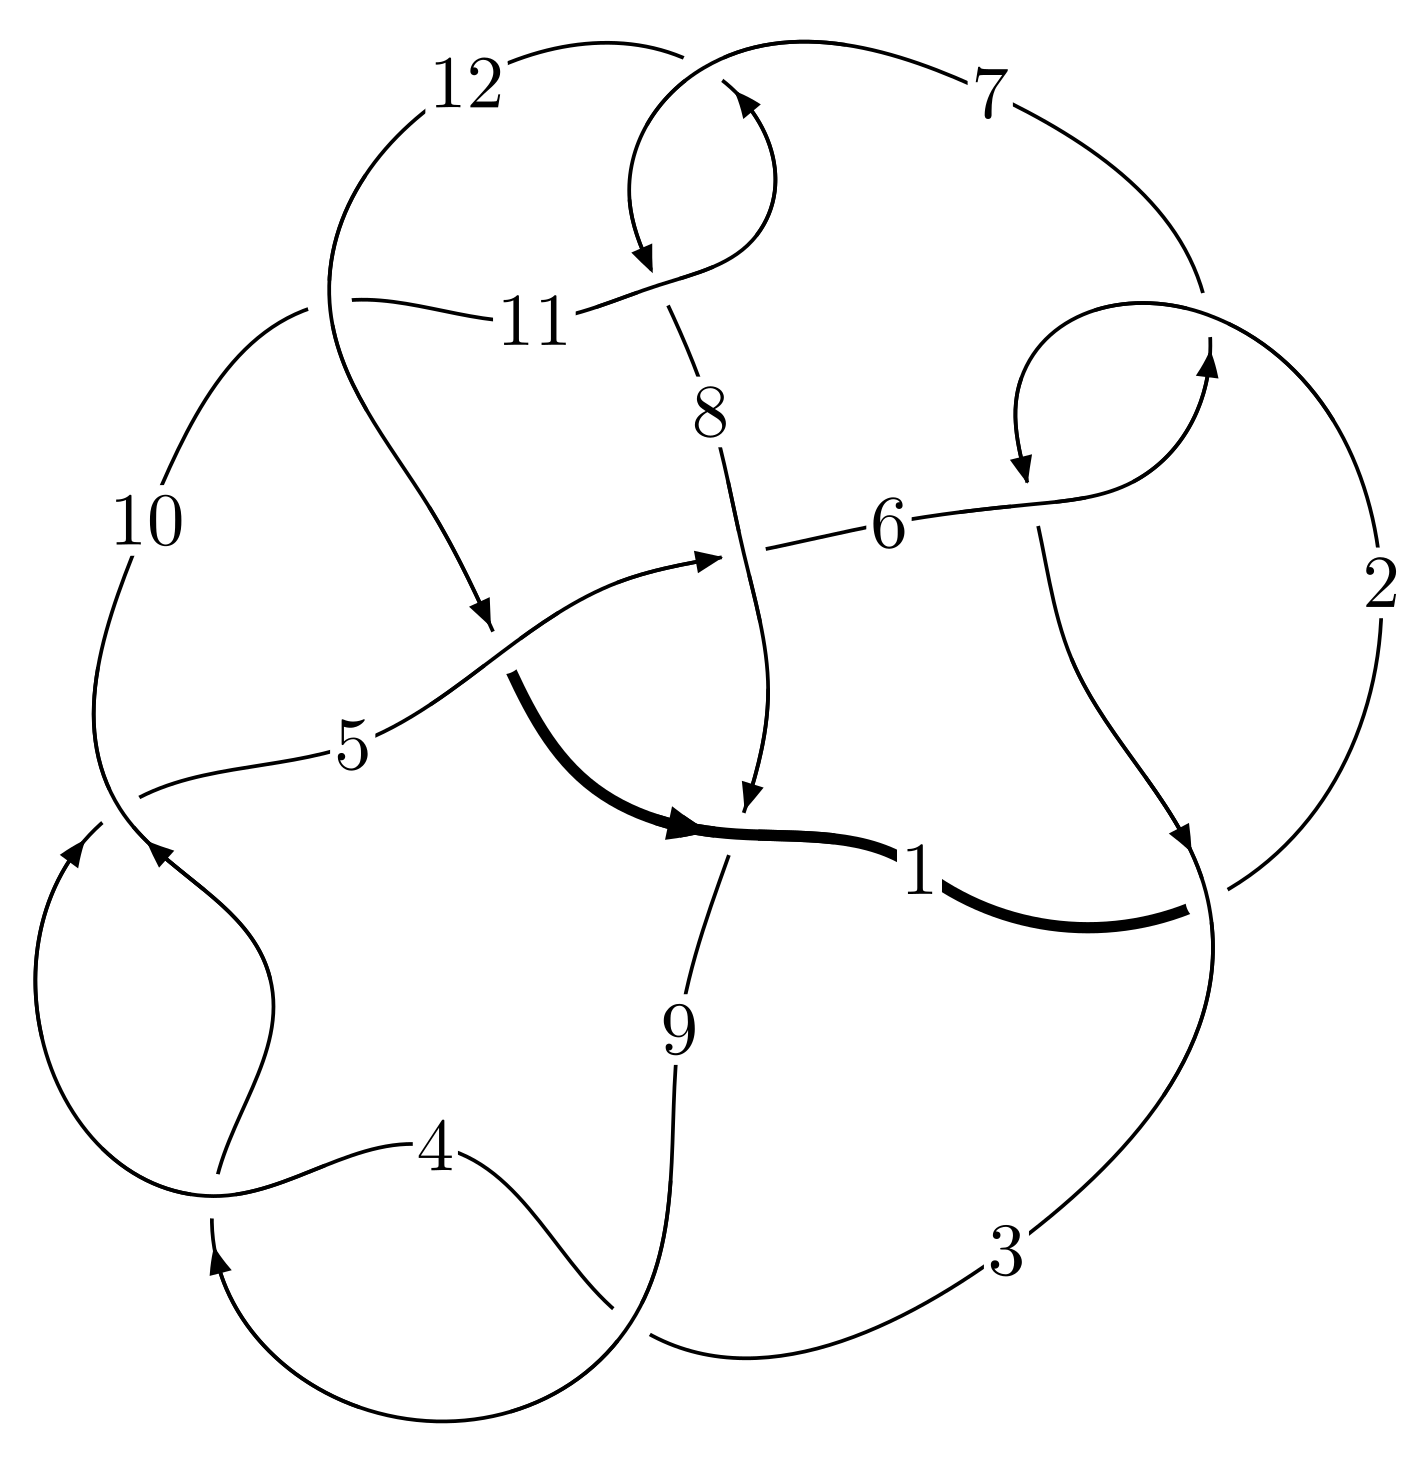
\includegraphics[width=112pt]{../../../GIT/diagram.site/Diagrams/png/1187_12a_0386.png}\\
\ \ \ A knot diagram\footnotemark}&
\allowdisplaybreaks
\textbf{Linearized knot diagam} \\
\cline{2-2}
 &
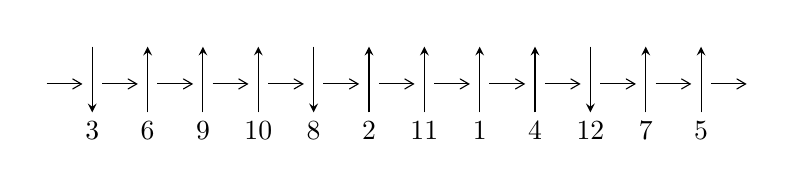
\begin{tikzpicture}[x=20pt, y=17pt]
	% nodes
	\node (C0) at (0, 0) {};
	\node (C1) at (1, 0) {};
	\node (C1U) at (1, +1) {};
	\node (C1D) at (1, -1) {3};

	\node (C2) at (2, 0) {};
	\node (C2U) at (2, +1) {};
	\node (C2D) at (2, -1) {6};

	\node (C3) at (3, 0) {};
	\node (C3U) at (3, +1) {};
	\node (C3D) at (3, -1) {9};

	\node (C4) at (4, 0) {};
	\node (C4U) at (4, +1) {};
	\node (C4D) at (4, -1) {10};

	\node (C5) at (5, 0) {};
	\node (C5U) at (5, +1) {};
	\node (C5D) at (5, -1) {8};

	\node (C6) at (6, 0) {};
	\node (C6U) at (6, +1) {};
	\node (C6D) at (6, -1) {2};

	\node (C7) at (7, 0) {};
	\node (C7U) at (7, +1) {};
	\node (C7D) at (7, -1) {11};

	\node (C8) at (8, 0) {};
	\node (C8U) at (8, +1) {};
	\node (C8D) at (8, -1) {1};

	\node (C9) at (9, 0) {};
	\node (C9U) at (9, +1) {};
	\node (C9D) at (9, -1) {4};

	\node (C10) at (10, 0) {};
	\node (C10U) at (10, +1) {};
	\node (C10D) at (10, -1) {12};

	\node (C11) at (11, 0) {};
	\node (C11U) at (11, +1) {};
	\node (C11D) at (11, -1) {7};

	\node (C12) at (12, 0) {};
	\node (C12U) at (12, +1) {};
	\node (C12D) at (12, -1) {5};
	\node (C13) at (13, 0) {};

	% arrows
	\draw[->,>={angle 60}]
	(C0) edge (C1) (C1) edge (C2) (C2) edge (C3) (C3) edge (C4) (C4) edge (C5) (C5) edge (C6) (C6) edge (C7) (C7) edge (C8) (C8) edge (C9) (C9) edge (C10) (C10) edge (C11) (C11) edge (C12) (C12) edge (C13) ;	\draw[->,>=stealth]
	(C1U) edge (C1D) (C2D) edge (C2U) (C3D) edge (C3U) (C4D) edge (C4U) (C5U) edge (C5D) (C6D) edge (C6U) (C7D) edge (C7U) (C8D) edge (C8U) (C9D) edge (C9U) (C10U) edge (C10D) (C11D) edge (C11U) (C12D) edge (C12U) ;
	\end{tikzpicture} \\
\hhline{~~} \\& 
\textbf{Solving Sequence} \\ \cline{2-2} 
 &
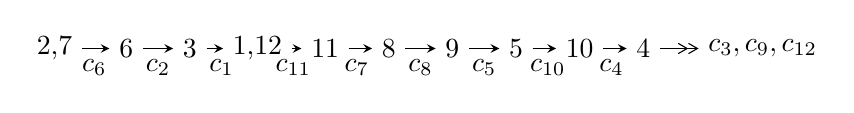
\begin{tikzpicture}[x=23pt, y=7pt]
	% node
	\node (A0) at (-1/8, 0) {2,7};
	\node (A1) at (1, 0) {6};
	\node (A2) at (2, 0) {3};
	\node (A3) at (49/16, 0) {1,12};
	\node (A4) at (33/8, 0) {11};
	\node (A5) at (41/8, 0) {8};
	\node (A6) at (49/8, 0) {9};
	\node (A7) at (57/8, 0) {5};
	\node (A8) at (65/8, 0) {10};
	\node (A9) at (73/8, 0) {4};
	\node (C1) at (1/2, -1) {$c_{6}$};
	\node (C2) at (3/2, -1) {$c_{2}$};
	\node (C3) at (5/2, -1) {$c_{1}$};
	\node (C4) at (29/8, -1) {$c_{11}$};
	\node (C5) at (37/8, -1) {$c_{7}$};
	\node (C6) at (45/8, -1) {$c_{8}$};
	\node (C7) at (53/8, -1) {$c_{5}$};
	\node (C8) at (61/8, -1) {$c_{10}$};
	\node (C9) at (69/8, -1) {$c_{4}$};
	\node (A10) at (11, 0) {$c_{3},c_{9},c_{12}$};

	% edge
	\draw[->,>=stealth]	
	(A0) edge (A1) (A1) edge (A2) (A2) edge (A3) (A3) edge (A4) (A4) edge (A5) (A5) edge (A6) (A6) edge (A7) (A7) edge (A8) (A8) edge (A9) ;
	\draw[->>,>={angle 60}]	
	(A9) edge (A10);
\end{tikzpicture} \\ 

\end{tabular} \\

\footnotetext{
The image of knot diagram is generated by the software ``\textbf{Draw programme}" developed by Andrew Bartholomew(\url{http://www.layer8.co.uk/maths/draw/index.htm\#Running-draw}), where we modified some parts for our purpose(\url{https://github.com/CATsTAILs/LinksPainter}).
}\phantom \\ \newline 
\centering \textbf{Ideals for irreducible components\footnotemark of $X_{\text{par}}$} 
 
\begin{align*}
I^u_{1}&=\langle 
b- u,\;-13623 u^{25}-12794 u^{24}+\cdots+24374 a+5797,\;u^{26}- u^{25}+\cdots+2 u-1\rangle \\
I^u_{2}&=\langle 
7.39786\times10^{132} u^{91}+1.99769\times10^{133} u^{90}+\cdots+5.07101\times10^{132} b-1.01915\times10^{133},\\
\phantom{I^u_{2}}&\phantom{= \langle  }-1.78004\times10^{132} u^{91}+4.64745\times10^{131} u^{90}+\cdots+2.53550\times10^{132} a-2.75480\times10^{133},\\
\phantom{I^u_{2}}&\phantom{= \langle  }u^{92}+2 u^{91}+\cdots+41 u+2\rangle \\
I^u_{3}&=\langle 
b+u,\;u^{11}+u^{10}+2 u^9+u^8+3 u^7+3 u^6+2 u^5+u^4+3 u^2+a,\\
\phantom{I^u_{3}}&\phantom{= \langle  }u^{12}+u^{11}+3 u^{10}+2 u^9+6 u^8+4 u^7+7 u^6+3 u^5+6 u^4+3 u^3+3 u^2+u+1\rangle \\
I^u_{4}&=\langle 
- u^{11}- u^{10}-3 u^9-2 u^8-6 u^7-4 u^6-7 u^5-4 u^4-6 u^3-2 u^2+b-3 u-1,\\
\phantom{I^u_{4}}&\phantom{= \langle  }u^{11}+u^{10}+2 u^9+u^8+3 u^7+3 u^6+2 u^5+2 u^4+u^2+a+1,\\
\phantom{I^u_{4}}&\phantom{= \langle  }u^{12}+u^{11}+3 u^{10}+2 u^9+6 u^8+4 u^7+7 u^6+4 u^5+6 u^4+2 u^3+3 u^2+u+1\rangle \\
\\
\end{align*}
\raggedright * 4 irreducible components of $\dim_{\mathbb{C}}=0$, with total 142 representations.\\
\footnotetext{All coefficients of polynomials are rational numbers. But the coefficients are sometimes approximated in decimal forms when there is not enough margin.}
\newpage
\renewcommand{\arraystretch}{1}
\centering \section*{I. $I^u_{1}= \langle b- u,\;-13623 u^{25}-12794 u^{24}+\cdots+24374 a+5797,\;u^{26}- u^{25}+\cdots+2 u-1 \rangle$}
\flushleft \textbf{(i) Arc colorings}\\
\begin{tabular}{m{7pt} m{180pt} m{7pt} m{180pt} }
\flushright $a_{2}=$&$\begin{pmatrix}0\\u\end{pmatrix}$ \\
\flushright $a_{7}=$&$\begin{pmatrix}1\\0\end{pmatrix}$ \\
\flushright $a_{6}=$&$\begin{pmatrix}1\\u^2\end{pmatrix}$ \\
\flushright $a_{3}=$&$\begin{pmatrix}u\\u^3+u\end{pmatrix}$ \\
\flushright $a_{1}=$&$\begin{pmatrix}u^3\\u^5+u^3+u\end{pmatrix}$ \\
\flushright $a_{12}=$&$\begin{pmatrix}0.558915 u^{25}+0.524904 u^{24}+\cdots-3.21010 u-0.237835\\u\end{pmatrix}$ \\
\flushright $a_{11}=$&$\begin{pmatrix}0.558915 u^{25}+0.524904 u^{24}+\cdots-4.21010 u-0.237835\\u\end{pmatrix}$ \\
\flushright $a_{8}=$&$\begin{pmatrix}-1.08382 u^{25}+0.646673 u^{24}+\cdots+1.35567 u+0.441085\\- u^2\end{pmatrix}$ \\
\flushright $a_{9}=$&$\begin{pmatrix}-0.785263 u^{25}+0.970296 u^{24}+\cdots+2.12210 u-0.0820546\\-0.102035 u^{25}-0.0894396 u^{24}+\cdots+0.193608 u+0.103758\end{pmatrix}$ \\
\flushright $a_{5}=$&$\begin{pmatrix}-0.677936 u^{25}+0.0100927 u^{24}+\cdots-0.814967 u+1.36490\\0.140108 u^{25}+0.375728 u^{24}+\cdots+1.05502 u-0.948265\end{pmatrix}$ \\
\flushright $a_{10}=$&$\begin{pmatrix}0.996061 u^{25}-0.753754 u^{24}+\cdots-5.81882 u+0.845983\\u^3+u\end{pmatrix}$ \\
\flushright $a_{4}=$&$\begin{pmatrix}-0.294617 u^{25}+0.430130 u^{24}+\cdots+4.05239 u-0.322844\\0.102035 u^{25}+0.0894396 u^{24}+\cdots-0.193608 u-0.103758\end{pmatrix}$\\&\end{tabular}
\flushleft \textbf{(ii) Obstruction class $= -1$}\\~\\
\flushleft \textbf{(iii) Cusp Shapes $= \frac{26279}{12187} u^{25}-\frac{14751}{12187} u^{24}+\cdots-\frac{2321}{12187} u+\frac{143807}{12187}$}\\~\\
\newpage\renewcommand{\arraystretch}{1}
\flushleft \textbf{(iv) u-Polynomials at the component}\newline \\
\begin{tabular}{m{50pt}|m{274pt}}
Crossings & \hspace{64pt}u-Polynomials at each crossing \\
\hline $$\begin{aligned}c_{1},c_{10}\end{aligned}$$&$\begin{aligned}
&u^{26}+11 u^{25}+\cdots-8 u+1
\end{aligned}$\\
\hline $$\begin{aligned}c_{2},c_{6},c_{7}\\c_{11}\end{aligned}$$&$\begin{aligned}
&u^{26}- u^{25}+\cdots+2 u-1
\end{aligned}$\\
\hline $$\begin{aligned}c_{3},c_{4},c_{9}\end{aligned}$$&$\begin{aligned}
&u^{26}+11 u^{25}+\cdots-8 u-32
\end{aligned}$\\
\hline $$\begin{aligned}c_{5}\end{aligned}$$&$\begin{aligned}
&u^{26}-24 u^{25}+\cdots-29184 u+2048
\end{aligned}$\\
\hline $$\begin{aligned}c_{8},c_{12}\end{aligned}$$&$\begin{aligned}
&u^{26}-6 u^{24}+\cdots+u-2
\end{aligned}$\\
\hline
\end{tabular}\\~\\
\newpage\renewcommand{\arraystretch}{1}
\flushleft \textbf{(v) Riley Polynomials at the component}\newline \\
\begin{tabular}{m{50pt}|m{274pt}}
Crossings & \hspace{64pt}Riley Polynomials at each crossing \\
\hline $$\begin{aligned}c_{1},c_{10}\end{aligned}$$&$\begin{aligned}
&y^{26}+15 y^{25}+\cdots-156 y+1
\end{aligned}$\\
\hline $$\begin{aligned}c_{2},c_{6},c_{7}\\c_{11}\end{aligned}$$&$\begin{aligned}
&y^{26}+11 y^{25}+\cdots-8 y+1
\end{aligned}$\\
\hline $$\begin{aligned}c_{3},c_{4},c_{9}\end{aligned}$$&$\begin{aligned}
&y^{26}-25 y^{25}+\cdots-1344 y+1024
\end{aligned}$\\
\hline $$\begin{aligned}c_{5}\end{aligned}$$&$\begin{aligned}
&y^{26}+58 y^{24}+\cdots-138674176 y+4194304
\end{aligned}$\\
\hline $$\begin{aligned}c_{8},c_{12}\end{aligned}$$&$\begin{aligned}
&y^{26}-12 y^{25}+\cdots+63 y+4
\end{aligned}$\\
\hline
\end{tabular}\\~\\
\newpage\flushleft \textbf{(vi) Complex Volumes and Cusp Shapes}
$$\begin{array}{c|c|c}  
\text{Solutions to }I^u_{1}& \I (\text{vol} + \sqrt{-1}CS) & \text{Cusp shape}\\
 \hline 
\begin{aligned}
u &= -0.807615 + 0.620588 I \\
a &= -1.41594 + 0.44568 I \\
b &= -0.807615 + 0.620588 I\end{aligned}
 & \phantom{-}4.61940 + 2.42366 I & \phantom{-}11.49135 - 1.87928 I \\ \hline\begin{aligned}
u &= -0.807615 - 0.620588 I \\
a &= -1.41594 - 0.44568 I \\
b &= -0.807615 - 0.620588 I\end{aligned}
 & \phantom{-}4.61940 - 2.42366 I & \phantom{-}11.49135 + 1.87928 I \\ \hline\begin{aligned}
u &= \phantom{-}0.685911 + 0.758379 I \\
a &= \phantom{-}1.50210 + 1.14201 I \\
b &= \phantom{-}0.685911 + 0.758379 I\end{aligned}
 & \phantom{-}2.96984 + 2.94472 I & \phantom{-}13.74154 - 2.94116 I \\ \hline\begin{aligned}
u &= \phantom{-}0.685911 - 0.758379 I \\
a &= \phantom{-}1.50210 - 1.14201 I \\
b &= \phantom{-}0.685911 - 0.758379 I\end{aligned}
 & \phantom{-}2.96984 - 2.94472 I & \phantom{-}13.74154 + 2.94116 I \\ \hline\begin{aligned}
u &= \phantom{-}0.329454 + 0.917116 I \\
a &= \phantom{-}2.49009 - 1.59537 I \\
b &= \phantom{-}0.329454 + 0.917116 I\end{aligned}
 & -2.86243 + 2.69103 I & \phantom{-}3.21966 - 6.77085 I \\ \hline\begin{aligned}
u &= \phantom{-}0.329454 - 0.917116 I \\
a &= \phantom{-}2.49009 + 1.59537 I \\
b &= \phantom{-}0.329454 - 0.917116 I\end{aligned}
 & -2.86243 - 2.69103 I & \phantom{-}3.21966 + 6.77085 I \\ \hline\begin{aligned}
u &= -0.664437 + 0.829427 I \\
a &= -3.39426 - 0.66607 I \\
b &= -0.664437 + 0.829427 I\end{aligned}
 & \phantom{-}9.68736 - 2.24802 I & \phantom{-}12.39075 + 4.49177 I \\ \hline\begin{aligned}
u &= -0.664437 - 0.829427 I \\
a &= -3.39426 + 0.66607 I \\
b &= -0.664437 - 0.829427 I\end{aligned}
 & \phantom{-}9.68736 + 2.24802 I & \phantom{-}12.39075 - 4.49177 I \\ \hline\begin{aligned}
u &= -0.144028 + 1.075630 I \\
a &= -0.93960 - 1.40239 I \\
b &= -0.144028 + 1.075630 I\end{aligned}
 & -5.86362 + 0.20015 I & -4.19232 - 0.64656 I \\ \hline\begin{aligned}
u &= -0.144028 - 1.075630 I \\
a &= -0.93960 + 1.40239 I \\
b &= -0.144028 - 1.075630 I\end{aligned}
 & -5.86362 - 0.20015 I & -4.19232 + 0.64656 I\\
 \hline 
 \end{array}$$\newpage$$\begin{array}{c|c|c}  
\text{Solutions to }I^u_{1}& \I (\text{vol} + \sqrt{-1}CS) & \text{Cusp shape}\\
 \hline 
\begin{aligned}
u &= \phantom{-}0.941091 + 0.622014 I \\
a &= \phantom{-}1.67976 + 0.31359 I \\
b &= \phantom{-}0.941091 + 0.622014 I\end{aligned}
 & \phantom{-}12.33100 - 5.65494 I & \phantom{-}13.25979 + 1.47273 I \\ \hline\begin{aligned}
u &= \phantom{-}0.941091 - 0.622014 I \\
a &= \phantom{-}1.67976 - 0.31359 I \\
b &= \phantom{-}0.941091 - 0.622014 I\end{aligned}
 & \phantom{-}12.33100 + 5.65494 I & \phantom{-}13.25979 - 1.47273 I \\ \hline\begin{aligned}
u &= -0.718112 + 0.900060 I \\
a &= -2.12467 + 0.83966 I \\
b &= -0.718112 + 0.900060 I\end{aligned}
 & \phantom{-}9.28845 - 8.45450 I & \phantom{-}12.1791 + 8.6146 I \\ \hline\begin{aligned}
u &= -0.718112 - 0.900060 I \\
a &= -2.12467 - 0.83966 I \\
b &= -0.718112 - 0.900060 I\end{aligned}
 & \phantom{-}9.28845 + 8.45450 I & \phantom{-}12.1791 - 8.6146 I \\ \hline\begin{aligned}
u &= \phantom{-}0.643874 + 0.975926 I \\
a &= \phantom{-}2.71464 - 1.15433 I \\
b &= \phantom{-}0.643874 + 0.975926 I\end{aligned}
 & \phantom{-}1.56867 + 7.39409 I & \phantom{-}9.80460 - 8.29279 I \\ \hline\begin{aligned}
u &= \phantom{-}0.643874 - 0.975926 I \\
a &= \phantom{-}2.71464 + 1.15433 I \\
b &= \phantom{-}0.643874 - 0.975926 I\end{aligned}
 & \phantom{-}1.56867 - 7.39409 I & \phantom{-}9.80460 + 8.29279 I \\ \hline\begin{aligned}
u &= \phantom{-}0.043255 + 1.216790 I \\
a &= \phantom{-}0.450845 - 0.826169 I \\
b &= \phantom{-}0.043255 + 1.216790 I\end{aligned}
 & -1.24232 - 2.12927 I & \phantom{-}4.01236 + 3.25160 I \\ \hline\begin{aligned}
u &= \phantom{-}0.043255 - 1.216790 I \\
a &= \phantom{-}0.450845 + 0.826169 I \\
b &= \phantom{-}0.043255 - 1.216790 I\end{aligned}
 & -1.24232 + 2.12927 I & \phantom{-}4.01236 - 3.25160 I \\ \hline\begin{aligned}
u &= \phantom{-}0.186488 + 0.738957 I \\
a &= -0.359062 - 0.571045 I \\
b &= \phantom{-}0.186488 + 0.738957 I\end{aligned}
 & -1.43325 + 1.76515 I & \phantom{-}5.03671 - 5.93425 I \\ \hline\begin{aligned}
u &= \phantom{-}0.186488 - 0.738957 I \\
a &= -0.359062 + 0.571045 I \\
b &= \phantom{-}0.186488 - 0.738957 I\end{aligned}
 & -1.43325 - 1.76515 I & \phantom{-}5.03671 + 5.93425 I\\
 \hline 
 \end{array}$$\newpage$$\begin{array}{c|c|c}  
\text{Solutions to }I^u_{1}& \I (\text{vol} + \sqrt{-1}CS) & \text{Cusp shape}\\
 \hline 
\begin{aligned}
u &= -0.688964 + 1.070760 I \\
a &= -2.23446 - 0.81457 I \\
b &= -0.688964 + 1.070760 I\end{aligned}
 & \phantom{-}1.85165 - 13.77330 I & \phantom{-}6.97647 + 10.67636 I \\ \hline\begin{aligned}
u &= -0.688964 - 1.070760 I \\
a &= -2.23446 + 0.81457 I \\
b &= -0.688964 - 1.070760 I\end{aligned}
 & \phantom{-}1.85165 + 13.77330 I & \phantom{-}6.97647 - 10.67636 I \\ \hline\begin{aligned}
u &= \phantom{-}0.752694 + 1.118140 I \\
a &= \phantom{-}2.15761 - 0.51442 I \\
b &= \phantom{-}0.752694 + 1.118140 I\end{aligned}
 & \phantom{-}9.2507 + 18.1776 I & \phantom{-}9.30289 - 9.71516 I \\ \hline\begin{aligned}
u &= \phantom{-}0.752694 - 1.118140 I \\
a &= \phantom{-}2.15761 + 0.51442 I \\
b &= \phantom{-}0.752694 - 1.118140 I\end{aligned}
 & \phantom{-}9.2507 - 18.1776 I & \phantom{-}9.30289 + 9.71516 I \\ \hline\begin{aligned}
u &= -0.417843\phantom{ +0.000000I} \\
a &= \phantom{-}3.42500\phantom{ +0.000000I} \\
b &= -0.417843\phantom{ +0.000000I}\end{aligned}
 & \phantom{-}7.84141\phantom{ +0.000000I} & \phantom{-}10.0650\phantom{ +0.000000I} \\ \hline\begin{aligned}
u &= \phantom{-}0.298624\phantom{ +0.000000I} \\
a &= -0.479073\phantom{ +0.000000I} \\
b &= \phantom{-}0.298624\phantom{ +0.000000I}\end{aligned}
 & \phantom{-}0.653973\phantom{ +0.000000I} & \phantom{-}15.4890\phantom{ +0.000000I}\\
 \hline 
 \end{array}$$\newpage\newpage\renewcommand{\arraystretch}{1}
\centering \section*{II. $I^u_{2}= \langle 7.40\times10^{132} u^{91}+2.00\times10^{133} u^{90}+\cdots+5.07\times10^{132} b-1.02\times10^{133},\;-1.78\times10^{132} u^{91}+4.65\times10^{131} u^{90}+\cdots+2.54\times10^{132} a-2.75\times10^{133},\;u^{92}+2 u^{91}+\cdots+41 u+2 \rangle$}
\flushleft \textbf{(i) Arc colorings}\\
\begin{tabular}{m{7pt} m{180pt} m{7pt} m{180pt} }
\flushright $a_{2}=$&$\begin{pmatrix}0\\u\end{pmatrix}$ \\
\flushright $a_{7}=$&$\begin{pmatrix}1\\0\end{pmatrix}$ \\
\flushright $a_{6}=$&$\begin{pmatrix}1\\u^2\end{pmatrix}$ \\
\flushright $a_{3}=$&$\begin{pmatrix}u\\u^3+u\end{pmatrix}$ \\
\flushright $a_{1}=$&$\begin{pmatrix}u^3\\u^5+u^3+u\end{pmatrix}$ \\
\flushright $a_{12}=$&$\begin{pmatrix}0.702046 u^{91}-0.183295 u^{90}+\cdots+154.391 u+10.8649\\-1.45885 u^{91}-3.93944 u^{90}+\cdots+25.5277 u+2.00976\end{pmatrix}$ \\
\flushright $a_{11}=$&$\begin{pmatrix}2.16090 u^{91}+3.75615 u^{90}+\cdots+128.863 u+8.85514\\-1.45885 u^{91}-3.93944 u^{90}+\cdots+25.5277 u+2.00976\end{pmatrix}$ \\
\flushright $a_{8}=$&$\begin{pmatrix}-3.09629 u^{91}-8.80027 u^{90}+\cdots-2.33000 u+4.74136\\-2.50890 u^{91}-5.76206 u^{90}+\cdots+44.4508 u+2.16426\end{pmatrix}$ \\
\flushright $a_{9}=$&$\begin{pmatrix}-7.54762 u^{91}-19.0382 u^{90}+\cdots+155.289 u+12.3751\\-4.02479 u^{91}-7.82729 u^{90}+\cdots+170.044 u+8.14333\end{pmatrix}$ \\
\flushright $a_{5}=$&$\begin{pmatrix}2.83666 u^{91}+4.59685 u^{90}+\cdots+45.4045 u+9.16643\\-1.97405 u^{91}-5.81218 u^{90}+\cdots+0.126535 u+1.64984\end{pmatrix}$ \\
\flushright $a_{10}=$&$\begin{pmatrix}-4.87434 u^{91}-12.3841 u^{90}+\cdots+343.215 u+9.88688\\-1.98056 u^{91}-4.31566 u^{90}+\cdots+93.1840 u+3.95306\end{pmatrix}$ \\
\flushright $a_{4}=$&$\begin{pmatrix}-1.99202 u^{91}+0.293742 u^{90}+\cdots+406.348 u+22.5493\\4.42433 u^{91}+15.5293 u^{90}+\cdots+114.784 u+5.48884\end{pmatrix}$\\&\end{tabular}
\flushleft \textbf{(ii) Obstruction class $= -1$}\\~\\
\flushleft \textbf{(iii) Cusp Shapes $= -11.6941 u^{91}-28.4552 u^{90}+\cdots+63.6053 u+5.57785$}\\~\\
\newpage\renewcommand{\arraystretch}{1}
\flushleft \textbf{(iv) u-Polynomials at the component}\newline \\
\begin{tabular}{m{50pt}|m{274pt}}
Crossings & \hspace{64pt}u-Polynomials at each crossing \\
\hline $$\begin{aligned}c_{1},c_{10}\end{aligned}$$&$\begin{aligned}
&u^{92}+32 u^{91}+\cdots-225 u+4
\end{aligned}$\\
\hline $$\begin{aligned}c_{2},c_{6},c_{7}\\c_{11}\end{aligned}$$&$\begin{aligned}
&u^{92}+2 u^{91}+\cdots+41 u+2
\end{aligned}$\\
\hline $$\begin{aligned}c_{3},c_{4},c_{9}\end{aligned}$$&$\begin{aligned}
&(u^{46}-5 u^{45}+\cdots- u+1)^{2}
\end{aligned}$\\
\hline $$\begin{aligned}c_{5}\end{aligned}$$&$\begin{aligned}
&(u^{46}+11 u^{45}+\cdots-11 u-1)^{2}
\end{aligned}$\\
\hline $$\begin{aligned}c_{8},c_{12}\end{aligned}$$&$\begin{aligned}
&u^{92}-5 u^{91}+\cdots-169896 u+138881
\end{aligned}$\\
\hline
\end{tabular}\\~\\
\newpage\renewcommand{\arraystretch}{1}
\flushleft \textbf{(v) Riley Polynomials at the component}\newline \\
\begin{tabular}{m{50pt}|m{274pt}}
Crossings & \hspace{64pt}Riley Polynomials at each crossing \\
\hline $$\begin{aligned}c_{1},c_{10}\end{aligned}$$&$\begin{aligned}
&y^{92}+60 y^{91}+\cdots+881743 y+16
\end{aligned}$\\
\hline $$\begin{aligned}c_{2},c_{6},c_{7}\\c_{11}\end{aligned}$$&$\begin{aligned}
&y^{92}+32 y^{91}+\cdots-225 y+4
\end{aligned}$\\
\hline $$\begin{aligned}c_{3},c_{4},c_{9}\end{aligned}$$&$\begin{aligned}
&(y^{46}-51 y^{45}+\cdots-43 y+1)^{2}
\end{aligned}$\\
\hline $$\begin{aligned}c_{5}\end{aligned}$$&$\begin{aligned}
&(y^{46}+11 y^{45}+\cdots+y+1)^{2}
\end{aligned}$\\
\hline $$\begin{aligned}c_{8},c_{12}\end{aligned}$$&$\begin{aligned}
&y^{92}-31 y^{91}+\cdots-535870573466 y+19287932161
\end{aligned}$\\
\hline
\end{tabular}\\~\\
\newpage\flushleft \textbf{(vi) Complex Volumes and Cusp Shapes}
$$\begin{array}{c|c|c}  
\text{Solutions to }I^u_{2}& \I (\text{vol} + \sqrt{-1}CS) & \text{Cusp shape}\\
 \hline 
\begin{aligned}
u &= \phantom{-}0.384275 + 0.922259 I \\
a &= -0.196400 - 0.647605 I \\
b &= -0.107571 + 0.785518 I\end{aligned}
 & -1.49826 + 1.86565 I & \phantom{-0.000000 } 0 \\ \hline\begin{aligned}
u &= \phantom{-}0.384275 - 0.922259 I \\
a &= -0.196400 + 0.647605 I \\
b &= -0.107571 - 0.785518 I\end{aligned}
 & -1.49826 - 1.86565 I & \phantom{-0.000000 } 0 \\ \hline\begin{aligned}
u &= \phantom{-}0.104954 + 0.988208 I \\
a &= \phantom{-}0.06006 + 1.83739 I \\
b &= \phantom{-}0.527133 - 0.897374 I\end{aligned}
 & -1.74949 - 1.99664 I & \phantom{-0.000000 } 0 \\ \hline\begin{aligned}
u &= \phantom{-}0.104954 - 0.988208 I \\
a &= \phantom{-}0.06006 - 1.83739 I \\
b &= \phantom{-}0.527133 + 0.897374 I\end{aligned}
 & -1.74949 + 1.99664 I & \phantom{-0.000000 } 0 \\ \hline\begin{aligned}
u &= \phantom{-}0.672129 + 0.755146 I \\
a &= -0.97156 + 1.44268 I \\
b &= -1.199970 + 0.386947 I\end{aligned}
 & \phantom{-}10.12620 + 0.27578 I & \phantom{-0.000000 } 0 \\ \hline\begin{aligned}
u &= \phantom{-}0.672129 - 0.755146 I \\
a &= -0.97156 - 1.44268 I \\
b &= -1.199970 - 0.386947 I\end{aligned}
 & \phantom{-}10.12620 - 0.27578 I & \phantom{-0.000000 } 0 \\ \hline\begin{aligned}
u &= -0.845063 + 0.559528 I \\
a &= -1.40890 - 0.46109 I \\
b &= -0.693227 - 1.033110 I\end{aligned}
 & \phantom{-}3.38247 + 8.06038 I & \phantom{-0.000000 } 0 \\ \hline\begin{aligned}
u &= -0.845063 - 0.559528 I \\
a &= -1.40890 + 0.46109 I \\
b &= -0.693227 + 1.033110 I\end{aligned}
 & \phantom{-}3.38247 - 8.06038 I & \phantom{-0.000000 } 0 \\ \hline\begin{aligned}
u &= \phantom{-}0.894041 + 0.372500 I \\
a &= -1.172930 + 0.459245 I \\
b &= -0.633260 + 0.846876 I\end{aligned}
 & \phantom{-}3.07336 - 0.96915 I & \phantom{-0.000000 } 0 \\ \hline\begin{aligned}
u &= \phantom{-}0.894041 - 0.372500 I \\
a &= -1.172930 - 0.459245 I \\
b &= -0.633260 - 0.846876 I\end{aligned}
 & \phantom{-}3.07336 + 0.96915 I & \phantom{-0.000000 } 0\\
 \hline 
 \end{array}$$\newpage$$\begin{array}{c|c|c}  
\text{Solutions to }I^u_{2}& \I (\text{vol} + \sqrt{-1}CS) & \text{Cusp shape}\\
 \hline 
\begin{aligned}
u &= \phantom{-}0.527133 + 0.897374 I \\
a &= -1.08952 + 1.37635 I \\
b &= \phantom{-}0.104954 - 0.988208 I\end{aligned}
 & -1.74949 + 1.99664 I & \phantom{-0.000000 } 0 \\ \hline\begin{aligned}
u &= \phantom{-}0.527133 - 0.897374 I \\
a &= -1.08952 - 1.37635 I \\
b &= \phantom{-}0.104954 + 0.988208 I\end{aligned}
 & -1.74949 - 1.99664 I & \phantom{-0.000000 } 0 \\ \hline\begin{aligned}
u &= \phantom{-}0.657222 + 0.697436 I \\
a &= \phantom{-}1.98616 - 0.38406 I \\
b &= \phantom{-}0.671820 - 0.937942 I\end{aligned}
 & \phantom{-}2.42160 - 2.30364 I & \phantom{-0.000000 } 0 \\ \hline\begin{aligned}
u &= \phantom{-}0.657222 - 0.697436 I \\
a &= \phantom{-}1.98616 + 0.38406 I \\
b &= \phantom{-}0.671820 + 0.937942 I\end{aligned}
 & \phantom{-}2.42160 + 2.30364 I & \phantom{-0.000000 } 0 \\ \hline\begin{aligned}
u &= -0.641745 + 0.838715 I \\
a &= \phantom{-}1.44102 + 0.26317 I \\
b &= \phantom{-}0.917442 - 0.560673 I\end{aligned}
 & \phantom{-}3.10180 - 4.01845 I & \phantom{-0.000000 } 0 \\ \hline\begin{aligned}
u &= -0.641745 - 0.838715 I \\
a &= \phantom{-}1.44102 - 0.26317 I \\
b &= \phantom{-}0.917442 + 0.560673 I\end{aligned}
 & \phantom{-}3.10180 + 4.01845 I & \phantom{-0.000000 } 0 \\ \hline\begin{aligned}
u &= -0.633260 + 0.846876 I \\
a &= \phantom{-}0.670798 + 0.938661 I \\
b &= \phantom{-}0.894041 + 0.372500 I\end{aligned}
 & \phantom{-}3.07336 - 0.96915 I & \phantom{-0.000000 } 0 \\ \hline\begin{aligned}
u &= -0.633260 - 0.846876 I \\
a &= \phantom{-}0.670798 - 0.938661 I \\
b &= \phantom{-}0.894041 - 0.372500 I\end{aligned}
 & \phantom{-}3.07336 + 0.96915 I & \phantom{-0.000000 } 0 \\ \hline\begin{aligned}
u &= \phantom{-}0.138860 + 1.051530 I \\
a &= -0.181379 - 0.286249 I \\
b &= -0.517894 + 0.472786 I\end{aligned}
 & -1.73726 + 1.92631 I & \phantom{-0.000000 } 0 \\ \hline\begin{aligned}
u &= \phantom{-}0.138860 - 1.051530 I \\
a &= -0.181379 + 0.286249 I \\
b &= -0.517894 - 0.472786 I\end{aligned}
 & -1.73726 - 1.92631 I & \phantom{-0.000000 } 0\\
 \hline 
 \end{array}$$\newpage$$\begin{array}{c|c|c}  
\text{Solutions to }I^u_{2}& \I (\text{vol} + \sqrt{-1}CS) & \text{Cusp shape}\\
 \hline 
\begin{aligned}
u &= \phantom{-}0.651474 + 0.855223 I \\
a &= -0.722091 + 1.065280 I \\
b &= -0.87344 + 1.16989 I\end{aligned}
 & \phantom{-}7.65487 - 2.41625 I & \phantom{-0.000000 } 0 \\ \hline\begin{aligned}
u &= \phantom{-}0.651474 - 0.855223 I \\
a &= -0.722091 - 1.065280 I \\
b &= -0.87344 - 1.16989 I\end{aligned}
 & \phantom{-}7.65487 + 2.41625 I & \phantom{-0.000000 } 0 \\ \hline\begin{aligned}
u &= \phantom{-}0.917442 + 0.560673 I \\
a &= -1.41331 - 0.26957 I \\
b &= -0.641745 - 0.838715 I\end{aligned}
 & \phantom{-}3.10180 + 4.01845 I & \phantom{-0.000000 } 0 \\ \hline\begin{aligned}
u &= \phantom{-}0.917442 - 0.560673 I \\
a &= -1.41331 + 0.26957 I \\
b &= -0.641745 + 0.838715 I\end{aligned}
 & \phantom{-}3.10180 - 4.01845 I & \phantom{-0.000000 } 0 \\ \hline\begin{aligned}
u &= \phantom{-}0.647081 + 0.859138 I \\
a &= -2.46993 + 0.50078 I \\
b &= -0.83829 - 1.22663 I\end{aligned}
 & \phantom{-}7.64236 + 7.46930 I & \phantom{-0.000000 } 0 \\ \hline\begin{aligned}
u &= \phantom{-}0.647081 - 0.859138 I \\
a &= -2.46993 - 0.50078 I \\
b &= -0.83829 + 1.22663 I\end{aligned}
 & \phantom{-}7.64236 - 7.46930 I & \phantom{-0.000000 } 0 \\ \hline\begin{aligned}
u &= \phantom{-}0.668613 + 0.872921 I \\
a &= -0.516254 + 0.171332 I \\
b &= -0.0592993 + 0.0462954 I\end{aligned}
 & \phantom{-}1.01357 + 2.58423 I & \phantom{-0.000000 } 0 \\ \hline\begin{aligned}
u &= \phantom{-}0.668613 - 0.872921 I \\
a &= -0.516254 - 0.171332 I \\
b &= -0.0592993 - 0.0462954 I\end{aligned}
 & \phantom{-}1.01357 - 2.58423 I & \phantom{-0.000000 } 0 \\ \hline\begin{aligned}
u &= -0.737043 + 0.826535 I \\
a &= -0.63108 - 2.02908 I \\
b &= -0.669007 - 0.884235 I\end{aligned}
 & \phantom{-}9.51681 + 2.91709 I & \phantom{-0.000000 } 0 \\ \hline\begin{aligned}
u &= -0.737043 - 0.826535 I \\
a &= -0.63108 + 2.02908 I \\
b &= -0.669007 + 0.884235 I\end{aligned}
 & \phantom{-}9.51681 - 2.91709 I & \phantom{-0.000000 } 0\\
 \hline 
 \end{array}$$\newpage$$\begin{array}{c|c|c}  
\text{Solutions to }I^u_{2}& \I (\text{vol} + \sqrt{-1}CS) & \text{Cusp shape}\\
 \hline 
\begin{aligned}
u &= -0.669007 + 0.884235 I \\
a &= -1.86616 - 1.01078 I \\
b &= -0.737043 - 0.826535 I\end{aligned}
 & \phantom{-}9.51681 - 2.91709 I & \phantom{-0.000000 } 0 \\ \hline\begin{aligned}
u &= -0.669007 - 0.884235 I \\
a &= -1.86616 + 1.01078 I \\
b &= -0.737043 + 0.826535 I\end{aligned}
 & \phantom{-}9.51681 + 2.91709 I & \phantom{-0.000000 } 0 \\ \hline\begin{aligned}
u &= -0.568462 + 0.683326 I \\
a &= \phantom{-}0.734078 + 0.955365 I \\
b &= \phantom{-}0.770591 + 1.030330 I\end{aligned}
 & \phantom{-}1.73892 + 2.14972 I & \phantom{-0.000000 } 0 \\ \hline\begin{aligned}
u &= -0.568462 - 0.683326 I \\
a &= \phantom{-}0.734078 - 0.955365 I \\
b &= \phantom{-}0.770591 - 1.030330 I\end{aligned}
 & \phantom{-}1.73892 - 2.14972 I & \phantom{-0.000000 } 0 \\ \hline\begin{aligned}
u &= \phantom{-}0.773550 + 0.436944 I \\
a &= \phantom{-}0.292921 + 0.784690 I \\
b &= -0.243248 + 1.241290 I\end{aligned}
 & \phantom{-}4.40684 - 4.36446 I & \phantom{-0.000000 } 0 \\ \hline\begin{aligned}
u &= \phantom{-}0.773550 - 0.436944 I \\
a &= \phantom{-}0.292921 - 0.784690 I \\
b &= -0.243248 - 1.241290 I\end{aligned}
 & \phantom{-}4.40684 + 4.36446 I & \phantom{-0.000000 } 0 \\ \hline\begin{aligned}
u &= -0.898218 + 0.678865 I \\
a &= \phantom{-}0.179251 + 0.632745 I \\
b &= \phantom{-}0.014143 + 0.836013 I\end{aligned}
 & \phantom{-}5.97757 - 0.66120 I & \phantom{-0.000000 } 0 \\ \hline\begin{aligned}
u &= -0.898218 - 0.678865 I \\
a &= \phantom{-}0.179251 - 0.632745 I \\
b &= \phantom{-}0.014143 - 0.836013 I\end{aligned}
 & \phantom{-}5.97757 + 0.66120 I & \phantom{-0.000000 } 0 \\ \hline\begin{aligned}
u &= -0.585246 + 0.976451 I \\
a &= \phantom{-}1.99761 + 0.67960 I \\
b &= \phantom{-}0.692044 - 1.145060 I\end{aligned}
 & \phantom{-}0.81481 - 6.80898 I & \phantom{-0.000000 } 0 \\ \hline\begin{aligned}
u &= -0.585246 - 0.976451 I \\
a &= \phantom{-}1.99761 - 0.67960 I \\
b &= \phantom{-}0.692044 + 1.145060 I\end{aligned}
 & \phantom{-}0.81481 + 6.80898 I & \phantom{-0.000000 } 0\\
 \hline 
 \end{array}$$\newpage$$\begin{array}{c|c|c}  
\text{Solutions to }I^u_{2}& \I (\text{vol} + \sqrt{-1}CS) & \text{Cusp shape}\\
 \hline 
\begin{aligned}
u &= \phantom{-}0.659061 + 0.934255 I \\
a &= -1.62301 + 0.40053 I \\
b &= -1.208270 - 0.529614 I\end{aligned}
 & \phantom{-}9.57845 + 4.88836 I & \phantom{-0.000000 } 0 \\ \hline\begin{aligned}
u &= \phantom{-}0.659061 - 0.934255 I \\
a &= -1.62301 - 0.40053 I \\
b &= -1.208270 + 0.529614 I\end{aligned}
 & \phantom{-}9.57845 - 4.88836 I & \phantom{-0.000000 } 0 \\ \hline\begin{aligned}
u &= \phantom{-}0.671820 + 0.937942 I \\
a &= -0.00420 - 1.68031 I \\
b &= \phantom{-}0.657222 - 0.697436 I\end{aligned}
 & \phantom{-}2.42160 + 2.30364 I & \phantom{-0.000000 } 0 \\ \hline\begin{aligned}
u &= \phantom{-}0.671820 - 0.937942 I \\
a &= -0.00420 + 1.68031 I \\
b &= \phantom{-}0.657222 + 0.697436 I\end{aligned}
 & \phantom{-}2.42160 - 2.30364 I & \phantom{-0.000000 } 0 \\ \hline\begin{aligned}
u &= \phantom{-}0.993762 + 0.598379 I \\
a &= \phantom{-}1.33362 - 0.67978 I \\
b &= \phantom{-}0.742562 - 1.087310 I\end{aligned}
 & \phantom{-}10.8811 - 11.8282 I & \phantom{-0.000000 } 0 \\ \hline\begin{aligned}
u &= \phantom{-}0.993762 - 0.598379 I \\
a &= \phantom{-}1.33362 + 0.67978 I \\
b &= \phantom{-}0.742562 + 1.087310 I\end{aligned}
 & \phantom{-}10.8811 + 11.8282 I & \phantom{-0.000000 } 0 \\ \hline\begin{aligned}
u &= \phantom{-}0.014143 + 0.836013 I \\
a &= -0.546063 + 0.697155 I \\
b &= -0.898218 + 0.678865 I\end{aligned}
 & \phantom{-}5.97757 - 0.66120 I & \phantom{-}6.00000 + 0. I\phantom{ +0.000000I} \\ \hline\begin{aligned}
u &= \phantom{-}0.014143 - 0.836013 I \\
a &= -0.546063 - 0.697155 I \\
b &= -0.898218 - 0.678865 I\end{aligned}
 & \phantom{-}5.97757 + 0.66120 I & \phantom{-}6.00000 + 0. I\phantom{ +0.000000I} \\ \hline\begin{aligned}
u &= -0.586521 + 1.010100 I \\
a &= \phantom{-}1.119650 + 0.692976 I \\
b &= \phantom{-}0.075243 - 1.202660 I\end{aligned}
 & -3.13888 - 6.52644 I & \phantom{-0.000000 } 0 \\ \hline\begin{aligned}
u &= -0.586521 - 1.010100 I \\
a &= \phantom{-}1.119650 - 0.692976 I \\
b &= \phantom{-}0.075243 + 1.202660 I\end{aligned}
 & -3.13888 + 6.52644 I & \phantom{-0.000000 } 0\\
 \hline 
 \end{array}$$\newpage$$\begin{array}{c|c|c}  
\text{Solutions to }I^u_{2}& \I (\text{vol} + \sqrt{-1}CS) & \text{Cusp shape}\\
 \hline 
\begin{aligned}
u &= \phantom{-}0.075243 + 1.202660 I \\
a &= -0.670379 + 1.086120 I \\
b &= -0.586521 - 1.010100 I\end{aligned}
 & -3.13888 + 6.52644 I & \phantom{-0.000000 } 0 \\ \hline\begin{aligned}
u &= \phantom{-}0.075243 - 1.202660 I \\
a &= -0.670379 - 1.086120 I \\
b &= -0.586521 + 1.010100 I\end{aligned}
 & -3.13888 - 6.52644 I & \phantom{-0.000000 } 0 \\ \hline\begin{aligned}
u &= -0.107571 + 0.785518 I \\
a &= -0.626612 - 0.578450 I \\
b &= \phantom{-}0.384275 + 0.922259 I\end{aligned}
 & -1.49826 + 1.86565 I & \phantom{-}3.52037 - 4.33930 I \\ \hline\begin{aligned}
u &= -0.107571 - 0.785518 I \\
a &= -0.626612 + 0.578450 I \\
b &= \phantom{-}0.384275 - 0.922259 I\end{aligned}
 & -1.49826 - 1.86565 I & \phantom{-}3.52037 + 4.33930 I \\ \hline\begin{aligned}
u &= -0.693227 + 1.033110 I \\
a &= -0.382680 - 1.145400 I \\
b &= -0.845063 - 0.559528 I\end{aligned}
 & \phantom{-}3.38247 - 8.06038 I & \phantom{-0.000000 } 0 \\ \hline\begin{aligned}
u &= -0.693227 - 1.033110 I \\
a &= -0.382680 + 1.145400 I \\
b &= -0.845063 + 0.559528 I\end{aligned}
 & \phantom{-}3.38247 + 8.06038 I & \phantom{-0.000000 } 0 \\ \hline\begin{aligned}
u &= \phantom{-}0.634075 + 1.073450 I \\
a &= -1.232080 + 0.266868 I \\
b &= -0.216288 - 1.390700 I\end{aligned}
 & \phantom{-}2.60520 + 9.64233 I & \phantom{-0.000000 } 0 \\ \hline\begin{aligned}
u &= \phantom{-}0.634075 - 1.073450 I \\
a &= -1.232080 - 0.266868 I \\
b &= -0.216288 + 1.390700 I\end{aligned}
 & \phantom{-}2.60520 - 9.64233 I & \phantom{-0.000000 } 0 \\ \hline\begin{aligned}
u &= \phantom{-}0.282265 + 0.698034 I \\
a &= \phantom{-}0.85393 - 2.11174 I \\
b &= \phantom{-}0.282265 - 0.698034 I\end{aligned}
 & -1.99436\phantom{ +0.000000I} & \phantom{-}6.54077 + 0. I\phantom{ +0.000000I} \\ \hline\begin{aligned}
u &= \phantom{-}0.282265 - 0.698034 I \\
a &= \phantom{-}0.85393 + 2.11174 I \\
b &= \phantom{-}0.282265 + 0.698034 I\end{aligned}
 & -1.99436\phantom{ +0.000000I} & \phantom{-}6.54077 + 0. I\phantom{ +0.000000I}\\
 \hline 
 \end{array}$$\newpage$$\begin{array}{c|c|c}  
\text{Solutions to }I^u_{2}& \I (\text{vol} + \sqrt{-1}CS) & \text{Cusp shape}\\
 \hline 
\begin{aligned}
u &= -1.199970 + 0.386947 I \\
a &= \phantom{-}1.372760 + 0.245997 I \\
b &= \phantom{-}0.672129 + 0.755146 I\end{aligned}
 & \phantom{-}10.12620 + 0.27578 I & \phantom{-0.000000 } 0 \\ \hline\begin{aligned}
u &= -1.199970 - 0.386947 I \\
a &= \phantom{-}1.372760 - 0.245997 I \\
b &= \phantom{-}0.672129 - 0.755146 I\end{aligned}
 & \phantom{-}10.12620 - 0.27578 I & \phantom{-0.000000 } 0 \\ \hline\begin{aligned}
u &= -0.243248 + 1.241290 I \\
a &= \phantom{-}0.587897 - 0.021533 I \\
b &= \phantom{-}0.773550 + 0.436944 I\end{aligned}
 & \phantom{-}4.40684 - 4.36446 I & \phantom{-0.000000 } 0 \\ \hline\begin{aligned}
u &= -0.243248 - 1.241290 I \\
a &= \phantom{-}0.587897 + 0.021533 I \\
b &= \phantom{-}0.773550 - 0.436944 I\end{aligned}
 & \phantom{-}4.40684 + 4.36446 I & \phantom{-0.000000 } 0 \\ \hline\begin{aligned}
u &= \phantom{-}0.099062 + 0.726030 I \\
a &= -1.58207 + 0.49349 I \\
b &= -0.774589 - 1.024930 I\end{aligned}
 & \phantom{-}4.93750 + 5.50082 I & \phantom{-}6.95120 - 5.88210 I \\ \hline\begin{aligned}
u &= \phantom{-}0.099062 - 0.726030 I \\
a &= -1.58207 - 0.49349 I \\
b &= -0.774589 + 1.024930 I\end{aligned}
 & \phantom{-}4.93750 - 5.50082 I & \phantom{-}6.95120 + 5.88210 I \\ \hline\begin{aligned}
u &= -0.774589 + 1.024930 I \\
a &= \phantom{-}0.924639 - 0.196309 I \\
b &= \phantom{-}0.099062 - 0.726030 I\end{aligned}
 & \phantom{-}4.93750 - 5.50082 I & \phantom{-0.000000 } 0 \\ \hline\begin{aligned}
u &= -0.774589 - 1.024930 I \\
a &= \phantom{-}0.924639 + 0.196309 I \\
b &= \phantom{-}0.099062 + 0.726030 I\end{aligned}
 & \phantom{-}4.93750 + 5.50082 I & \phantom{-0.000000 } 0 \\ \hline\begin{aligned}
u &= \phantom{-}0.770591 + 1.030330 I \\
a &= -0.523962 + 0.646747 I \\
b &= -0.568462 + 0.683326 I\end{aligned}
 & \phantom{-}1.73892 + 2.14972 I & \phantom{-0.000000 } 0 \\ \hline\begin{aligned}
u &= \phantom{-}0.770591 - 1.030330 I \\
a &= -0.523962 - 0.646747 I \\
b &= -0.568462 - 0.683326 I\end{aligned}
 & \phantom{-}1.73892 - 2.14972 I & \phantom{-0.000000 } 0\\
 \hline 
 \end{array}$$\newpage$$\begin{array}{c|c|c}  
\text{Solutions to }I^u_{2}& \I (\text{vol} + \sqrt{-1}CS) & \text{Cusp shape}\\
 \hline 
\begin{aligned}
u &= -0.517894 + 0.472786 I \\
a &= -0.512074 - 0.022450 I \\
b &= \phantom{-}0.138860 + 1.051530 I\end{aligned}
 & -1.73726 + 1.92631 I & \phantom{-}3.89432 - 4.39576 I \\ \hline\begin{aligned}
u &= -0.517894 - 0.472786 I \\
a &= -0.512074 + 0.022450 I \\
b &= \phantom{-}0.138860 - 1.051530 I\end{aligned}
 & -1.73726 - 1.92631 I & \phantom{-}3.89432 + 4.39576 I \\ \hline\begin{aligned}
u &= \phantom{-}0.197229 + 0.661581 I \\
a &= \phantom{-}1.75065 - 0.31294 I \\
b &= -0.614599 + 1.163900 I\end{aligned}
 & \phantom{-}5.26525 - 4.46279 I & \phantom{-}2.29672 + 4.19886 I \\ \hline\begin{aligned}
u &= \phantom{-}0.197229 - 0.661581 I \\
a &= \phantom{-}1.75065 + 0.31294 I \\
b &= -0.614599 - 1.163900 I\end{aligned}
 & \phantom{-}5.26525 + 4.46279 I & \phantom{-}2.29672 - 4.19886 I \\ \hline\begin{aligned}
u &= -0.614599 + 1.163900 I \\
a &= \phantom{-}0.540716 - 0.760064 I \\
b &= \phantom{-}0.197229 + 0.661581 I\end{aligned}
 & \phantom{-}5.26525 - 4.46279 I & \phantom{-0.000000 } 0 \\ \hline\begin{aligned}
u &= -0.614599 - 1.163900 I \\
a &= \phantom{-}0.540716 + 0.760064 I \\
b &= \phantom{-}0.197229 - 0.661581 I\end{aligned}
 & \phantom{-}5.26525 + 4.46279 I & \phantom{-0.000000 } 0 \\ \hline\begin{aligned}
u &= \phantom{-}0.742562 + 1.087310 I \\
a &= \phantom{-}0.665074 - 1.138780 I \\
b &= \phantom{-}0.993762 - 0.598379 I\end{aligned}
 & \phantom{-}10.8811 + 11.8282 I & \phantom{-0.000000 } 0 \\ \hline\begin{aligned}
u &= \phantom{-}0.742562 - 1.087310 I \\
a &= \phantom{-}0.665074 + 1.138780 I \\
b &= \phantom{-}0.993762 + 0.598379 I\end{aligned}
 & \phantom{-}10.8811 - 11.8282 I & \phantom{-0.000000 } 0 \\ \hline\begin{aligned}
u &= -1.208270 + 0.529614 I \\
a &= \phantom{-}1.38348 - 0.43005 I \\
b &= \phantom{-}0.659061 - 0.934255 I\end{aligned}
 & \phantom{-}9.57845 - 4.88836 I & \phantom{-0.000000 } 0 \\ \hline\begin{aligned}
u &= -1.208270 - 0.529614 I \\
a &= \phantom{-}1.38348 + 0.43005 I \\
b &= \phantom{-}0.659061 + 0.934255 I\end{aligned}
 & \phantom{-}9.57845 + 4.88836 I & \phantom{-0.000000 } 0\\
 \hline 
 \end{array}$$\newpage$$\begin{array}{c|c|c}  
\text{Solutions to }I^u_{2}& \I (\text{vol} + \sqrt{-1}CS) & \text{Cusp shape}\\
 \hline 
\begin{aligned}
u &= \phantom{-}0.692044 + 1.145060 I \\
a &= -1.70181 + 0.57199 I \\
b &= -0.585246 - 0.976451 I\end{aligned}
 & \phantom{-}0.81481 + 6.80898 I & \phantom{-0.000000 } 0 \\ \hline\begin{aligned}
u &= \phantom{-}0.692044 - 1.145060 I \\
a &= -1.70181 - 0.57199 I \\
b &= -0.585246 + 0.976451 I\end{aligned}
 & \phantom{-}0.81481 - 6.80898 I & \phantom{-0.000000 } 0 \\ \hline\begin{aligned}
u &= -0.357390 + 0.546281 I \\
a &= \phantom{-}2.16190 + 3.30453 I \\
b &= -0.357390 - 0.546281 I\end{aligned}
 & \phantom{-}7.61775\phantom{ +0.000000I} & \phantom{-}4.49295 + 0. I\phantom{ +0.000000I} \\ \hline\begin{aligned}
u &= -0.357390 - 0.546281 I \\
a &= \phantom{-}2.16190 - 3.30453 I \\
b &= -0.357390 + 0.546281 I\end{aligned}
 & \phantom{-}7.61775\phantom{ +0.000000I} & \phantom{-}4.49295 + 0. I\phantom{ +0.000000I} \\ \hline\begin{aligned}
u &= -0.216288 + 1.390700 I \\
a &= \phantom{-}0.926336 + 0.623675 I \\
b &= \phantom{-}0.634075 - 1.073450 I\end{aligned}
 & \phantom{-}2.60520 - 9.64233 I & \phantom{-0.000000 } 0 \\ \hline\begin{aligned}
u &= -0.216288 - 1.390700 I \\
a &= \phantom{-}0.926336 - 0.623675 I \\
b &= \phantom{-}0.634075 + 1.073450 I\end{aligned}
 & \phantom{-}2.60520 + 9.64233 I & \phantom{-0.000000 } 0 \\ \hline\begin{aligned}
u &= -0.87344 + 1.16989 I \\
a &= \phantom{-}0.608052 + 0.726893 I \\
b &= \phantom{-}0.651474 + 0.855223 I\end{aligned}
 & \phantom{-}7.65487 - 2.41625 I & \phantom{-0.000000 } 0 \\ \hline\begin{aligned}
u &= -0.87344 - 1.16989 I \\
a &= \phantom{-}0.608052 - 0.726893 I \\
b &= \phantom{-}0.651474 - 0.855223 I\end{aligned}
 & \phantom{-}7.65487 + 2.41625 I & \phantom{-0.000000 } 0 \\ \hline\begin{aligned}
u &= -0.83829 + 1.22663 I \\
a &= \phantom{-}1.76949 + 0.44441 I \\
b &= \phantom{-}0.647081 - 0.859138 I\end{aligned}
 & \phantom{-}7.64236 - 7.46930 I & \phantom{-0.000000 } 0 \\ \hline\begin{aligned}
u &= -0.83829 - 1.22663 I \\
a &= \phantom{-}1.76949 - 0.44441 I \\
b &= \phantom{-}0.647081 + 0.859138 I\end{aligned}
 & \phantom{-}7.64236 + 7.46930 I & \phantom{-0.000000 } 0\\
 \hline 
 \end{array}$$\newpage$$\begin{array}{c|c|c}  
\text{Solutions to }I^u_{2}& \I (\text{vol} + \sqrt{-1}CS) & \text{Cusp shape}\\
 \hline 
\begin{aligned}
u &= -0.0592993 + 0.0462954 I \\
a &= \phantom{-}2.43438 + 7.56829 I \\
b &= \phantom{-}0.668613 + 0.872921 I\end{aligned}
 & \phantom{-}1.01357 + 2.58423 I & \phantom{-}2.71428 - 4.03968 I \\ \hline\begin{aligned}
u &= -0.0592993 - 0.0462954 I \\
a &= \phantom{-}2.43438 - 7.56829 I \\
b &= \phantom{-}0.668613 - 0.872921 I\end{aligned}
 & \phantom{-}1.01357 - 2.58423 I & \phantom{-}2.71428 + 4.03968 I\\
 \hline 
 \end{array}$$\newpage\newpage\renewcommand{\arraystretch}{1}
\centering \section*{III. $I^u_{3}= \langle b+u,\;u^{11}+u^{10}+\cdots+3 u^2+a,\;u^{12}+u^{11}+\cdots+u+1 \rangle$}
\flushleft \textbf{(i) Arc colorings}\\
\begin{tabular}{m{7pt} m{180pt} m{7pt} m{180pt} }
\flushright $a_{2}=$&$\begin{pmatrix}0\\u\end{pmatrix}$ \\
\flushright $a_{7}=$&$\begin{pmatrix}1\\0\end{pmatrix}$ \\
\flushright $a_{6}=$&$\begin{pmatrix}1\\u^2\end{pmatrix}$ \\
\flushright $a_{3}=$&$\begin{pmatrix}u\\u^3+u\end{pmatrix}$ \\
\flushright $a_{1}=$&$\begin{pmatrix}u^3\\u^5+u^3+u\end{pmatrix}$ \\
\flushright $a_{12}=$&$\begin{pmatrix}- u^{11}- u^{10}-2 u^9- u^8-3 u^7-3 u^6-2 u^5- u^4-3 u^2\\- u\end{pmatrix}$ \\
\flushright $a_{11}=$&$\begin{pmatrix}- u^{11}- u^{10}-2 u^9- u^8-3 u^7-3 u^6-2 u^5- u^4-3 u^2+u\\- u\end{pmatrix}$ \\
\flushright $a_{8}=$&$\begin{pmatrix}u^{10}+u^9+3 u^8+u^7+5 u^6+2 u^5+6 u^4+4 u^2+u+2\\- u^2\end{pmatrix}$ \\
\flushright $a_{9}=$&$\begin{pmatrix}u^{10}+u^9+3 u^8+u^7+6 u^6+2 u^5+7 u^4+5 u^2+u+2\\u^8+2 u^6+3 u^4+u^2+1\end{pmatrix}$ \\
\flushright $a_{5}=$&$\begin{pmatrix}- u^{10}- u^9-3 u^8-2 u^7-6 u^6-4 u^5-7 u^4-2 u^3-5 u^2-2 u-2\\u^{11}+u^{10}+2 u^9+u^8+3 u^7+2 u^6+2 u^5+u^3+2 u^2\end{pmatrix}$ \\
\flushright $a_{10}=$&$\begin{pmatrix}u^9+2 u^7- u^6+4 u^5- u^4+3 u^3-2 u^2+2 u\\- u^3- u\end{pmatrix}$ \\
\flushright $a_{4}=$&$\begin{pmatrix}- u^{11}-3 u^9-6 u^7-7 u^5-6 u^3+u^2-3 u\\- u^8-2 u^6-3 u^4- u^2-1\end{pmatrix}$\\&\end{tabular}
\flushleft \textbf{(ii) Obstruction class $= 1$}\\~\\
\flushleft \textbf{(iii) Cusp Shapes $= 7 u^{11}+4 u^{10}+16 u^9+4 u^8+31 u^7+7 u^6+26 u^5-5 u^4+23 u^3-3 u^2+u+3$}\\~\\
\newpage\renewcommand{\arraystretch}{1}
\flushleft \textbf{(iv) u-Polynomials at the component}\newline \\
\begin{tabular}{m{50pt}|m{274pt}}
Crossings & \hspace{64pt}u-Polynomials at each crossing \\
\hline $$\begin{aligned}c_{1},c_{10}\end{aligned}$$&$\begin{aligned}
&u^{12}-5 u^{11}+\cdots-5 u+1
\end{aligned}$\\
\hline $$\begin{aligned}c_{2},c_{7}\end{aligned}$$&$\begin{aligned}
&u^{12}- u^{11}+\cdots- u+1
\end{aligned}$\\
\hline $$\begin{aligned}c_{3},c_{4}\end{aligned}$$&$\begin{aligned}
&u^{12}+2 u^{11}+\cdots+2 u+1
\end{aligned}$\\
\hline $$\begin{aligned}c_{5}\end{aligned}$$&$\begin{aligned}
&u^{12}- u^{11}-2 u^9+4 u^6-2 u^5- u^4+3 u^2+2 u+1
\end{aligned}$\\
\hline $$\begin{aligned}c_{6},c_{11}\end{aligned}$$&$\begin{aligned}
&u^{12}+u^{11}+\cdots+u+1
\end{aligned}$\\
\hline $$\begin{aligned}c_{8},c_{12}\end{aligned}$$&$\begin{aligned}
&u^{12}- u^{10}- u^9-3 u^8+u^7+3 u^6+2 u^5+u^4-2 u^3- u^2+1
\end{aligned}$\\
\hline $$\begin{aligned}c_{9}\end{aligned}$$&$\begin{aligned}
&u^{12}-2 u^{11}+\cdots-2 u+1
\end{aligned}$\\
\hline
\end{tabular}\\~\\
\newpage\renewcommand{\arraystretch}{1}
\flushleft \textbf{(v) Riley Polynomials at the component}\newline \\
\begin{tabular}{m{50pt}|m{274pt}}
Crossings & \hspace{64pt}Riley Polynomials at each crossing \\
\hline $$\begin{aligned}c_{1},c_{10}\end{aligned}$$&$\begin{aligned}
&y^{12}+9 y^{11}+\cdots+5 y+1
\end{aligned}$\\
\hline $$\begin{aligned}c_{2},c_{6},c_{7}\\c_{11}\end{aligned}$$&$\begin{aligned}
&y^{12}+5 y^{11}+\cdots+5 y+1
\end{aligned}$\\
\hline $$\begin{aligned}c_{3},c_{4},c_{9}\end{aligned}$$&$\begin{aligned}
&y^{12}-14 y^{11}+\cdots+2 y+1
\end{aligned}$\\
\hline $$\begin{aligned}c_{5}\end{aligned}$$&$\begin{aligned}
&y^{12}- y^{11}+\cdots+2 y+1
\end{aligned}$\\
\hline $$\begin{aligned}c_{8},c_{12}\end{aligned}$$&$\begin{aligned}
&y^{12}-2 y^{11}+\cdots-2 y+1
\end{aligned}$\\
\hline
\end{tabular}\\~\\
\newpage\flushleft \textbf{(vi) Complex Volumes and Cusp Shapes}
$$\begin{array}{c|c|c}  
\text{Solutions to }I^u_{3}& \I (\text{vol} + \sqrt{-1}CS) & \text{Cusp shape}\\
 \hline 
\begin{aligned}
u &= \phantom{-}0.655102 + 0.736440 I \\
a &= -1.251530 - 0.398490 I \\
b &= -0.655102 - 0.736440 I\end{aligned}
 & \phantom{-}1.97845 + 3.67934 I & \phantom{-}6.30875 - 7.16034 I \\ \hline\begin{aligned}
u &= \phantom{-}0.655102 - 0.736440 I \\
a &= -1.251530 + 0.398490 I \\
b &= -0.655102 + 0.736440 I\end{aligned}
 & \phantom{-}1.97845 - 3.67934 I & \phantom{-}6.30875 + 7.16034 I \\ \hline\begin{aligned}
u &= -0.793413 + 0.890052 I \\
a &= \phantom{-}2.01108 - 0.02373 I \\
b &= \phantom{-}0.793413 - 0.890052 I\end{aligned}
 & \phantom{-}8.13868 - 5.95932 I & \phantom{-}11.90060 + 5.23042 I \\ \hline\begin{aligned}
u &= -0.793413 - 0.890052 I \\
a &= \phantom{-}2.01108 + 0.02373 I \\
b &= \phantom{-}0.793413 + 0.890052 I\end{aligned}
 & \phantom{-}8.13868 + 5.95932 I & \phantom{-}11.90060 - 5.23042 I \\ \hline\begin{aligned}
u &= \phantom{-}0.592825 + 1.034570 I \\
a &= -1.95190 + 0.82796 I \\
b &= -0.592825 - 1.034570 I\end{aligned}
 & \phantom{-}0.03780 + 6.13395 I & \phantom{-}3.34772 - 4.32128 I \\ \hline\begin{aligned}
u &= \phantom{-}0.592825 - 1.034570 I \\
a &= -1.95190 - 0.82796 I \\
b &= -0.592825 + 1.034570 I\end{aligned}
 & \phantom{-}0.03780 - 6.13395 I & \phantom{-}3.34772 + 4.32128 I \\ \hline\begin{aligned}
u &= -0.554835 + 0.511693 I \\
a &= \phantom{-}0.11463 + 1.76794 I \\
b &= \phantom{-}0.554835 - 0.511693 I\end{aligned}
 & \phantom{-}8.17744 - 0.96019 I & \phantom{-}12.36505 + 4.95398 I \\ \hline\begin{aligned}
u &= -0.554835 - 0.511693 I \\
a &= \phantom{-}0.11463 - 1.76794 I \\
b &= \phantom{-}0.554835 + 0.511693 I\end{aligned}
 & \phantom{-}8.17744 + 0.96019 I & \phantom{-}12.36505 - 4.95398 I \\ \hline\begin{aligned}
u &= \phantom{-}0.147187 + 0.720863 I \\
a &= \phantom{-}1.32897 - 0.99098 I \\
b &= -0.147187 - 0.720863 I\end{aligned}
 & -2.42991 + 1.27964 I & \phantom{-}0.05150 - 3.21690 I \\ \hline\begin{aligned}
u &= \phantom{-}0.147187 - 0.720863 I \\
a &= \phantom{-}1.32897 + 0.99098 I \\
b &= -0.147187 + 0.720863 I\end{aligned}
 & -2.42991 - 1.27964 I & \phantom{-}0.05150 + 3.21690 I\\
 \hline 
 \end{array}$$\newpage$$\begin{array}{c|c|c}  
\text{Solutions to }I^u_{3}& \I (\text{vol} + \sqrt{-1}CS) & \text{Cusp shape}\\
 \hline 
\begin{aligned}
u &= -0.546865 + 1.162890 I \\
a &= \phantom{-}1.248760 + 0.553949 I \\
b &= \phantom{-}0.546865 - 1.162890 I\end{aligned}
 & \phantom{-}3.83675 - 8.25339 I & \phantom{-}10.02638 + 7.06157 I \\ \hline\begin{aligned}
u &= -0.546865 - 1.162890 I \\
a &= \phantom{-}1.248760 - 0.553949 I \\
b &= \phantom{-}0.546865 + 1.162890 I\end{aligned}
 & \phantom{-}3.83675 + 8.25339 I & \phantom{-}10.02638 - 7.06157 I\\
 \hline 
 \end{array}$$\newpage\newpage\renewcommand{\arraystretch}{1}
\centering \section*{IV. $I^u_{4}= \langle - u^{11}- u^{10}+\cdots+b-1,\;u^{11}+u^{10}+\cdots+a+1,\;u^{12}+u^{11}+\cdots+u+1 \rangle$}
\flushleft \textbf{(i) Arc colorings}\\
\begin{tabular}{m{7pt} m{180pt} m{7pt} m{180pt} }
\flushright $a_{2}=$&$\begin{pmatrix}0\\u\end{pmatrix}$ \\
\flushright $a_{7}=$&$\begin{pmatrix}1\\0\end{pmatrix}$ \\
\flushright $a_{6}=$&$\begin{pmatrix}1\\u^2\end{pmatrix}$ \\
\flushright $a_{3}=$&$\begin{pmatrix}u\\u^3+u\end{pmatrix}$ \\
\flushright $a_{1}=$&$\begin{pmatrix}u^3\\u^5+u^3+u\end{pmatrix}$ \\
\flushright $a_{12}=$&$\begin{pmatrix}- u^{11}- u^{10}-2 u^9- u^8-3 u^7-3 u^6-2 u^5-2 u^4- u^2-1\\u^{11}+u^{10}+3 u^9+2 u^8+6 u^7+4 u^6+7 u^5+4 u^4+6 u^3+2 u^2+3 u+1\end{pmatrix}$ \\
\flushright $a_{11}=$&$\begin{pmatrix}-2 u^{11}-2 u^{10}+\cdots-3 u-2\\u^{11}+u^{10}+3 u^9+2 u^8+6 u^7+4 u^6+7 u^5+4 u^4+6 u^3+2 u^2+3 u+1\end{pmatrix}$ \\
\flushright $a_{8}=$&$\begin{pmatrix}2 u^{11}+4 u^9- u^8+9 u^7- u^6+7 u^5- u^4+6 u^3-2 u^2+3 u\\- u^{11}-2 u^9+u^8-4 u^7+2 u^6-3 u^5+3 u^4-2 u^3+4 u^2- u+2\end{pmatrix}$ \\
\flushright $a_{9}=$&$\begin{pmatrix}2 u^{11}+4 u^9- u^8+9 u^7- u^6+7 u^5+6 u^3- u^2+3 u+1\\u^6+2 u^4+3 u^2+2\end{pmatrix}$ \\
\flushright $a_{5}=$&$\begin{pmatrix}- u^{10}- u^9-3 u^8-2 u^7-6 u^6-4 u^5-7 u^4-3 u^3-5 u^2- u-2\\u^{11}+u^{10}+2 u^9+u^8+3 u^7+2 u^6+2 u^5+u^4+u^3+1\end{pmatrix}$ \\
\flushright $a_{10}=$&$\begin{pmatrix}-3 u^{11}-2 u^{10}+\cdots-4 u-1\\- u^{11}-2 u^{10}-3 u^9-4 u^8-5 u^7-8 u^6-5 u^5-7 u^4-3 u^3-4 u^2+u-2\end{pmatrix}$ \\
\flushright $a_{4}=$&$\begin{pmatrix}-2 u^{11}-2 u^{10}+\cdots-4 u-2\\u^{11}- u^{10}+2 u^9-3 u^8+4 u^7-6 u^6+3 u^5-5 u^4+u^3-4 u^2+2 u-2\end{pmatrix}$\\&\end{tabular}
\flushleft \textbf{(ii) Obstruction class $= 1$}\\~\\
\flushleft \textbf{(iii) Cusp Shapes $= 5 u^{11}+7 u^{10}+13 u^9+11 u^8+23 u^7+23 u^6+21 u^5+15 u^4+17 u^3+8 u^2+12$}\\~\\
\newpage\renewcommand{\arraystretch}{1}
\flushleft \textbf{(iv) u-Polynomials at the component}\newline \\
\begin{tabular}{m{50pt}|m{274pt}}
Crossings & \hspace{64pt}u-Polynomials at each crossing \\
\hline $$\begin{aligned}c_{1},c_{10}\end{aligned}$$&$\begin{aligned}
&u^{12}-5 u^{11}+\cdots-5 u+1
\end{aligned}$\\
\hline $$\begin{aligned}c_{2},c_{7}\end{aligned}$$&$\begin{aligned}
&u^{12}- u^{11}+\cdots- u+1
\end{aligned}$\\
\hline $$\begin{aligned}c_{3},c_{4}\end{aligned}$$&$\begin{aligned}
&(u^6- u^5-3 u^4+3 u^3+u^2- u+1)^2
\end{aligned}$\\
\hline $$\begin{aligned}c_{5}\end{aligned}$$&$\begin{aligned}
&(u^6- u^5+u^4+u^3- u^2+u-1)^2
\end{aligned}$\\
\hline $$\begin{aligned}c_{6},c_{11}\end{aligned}$$&$\begin{aligned}
&u^{12}+u^{11}+\cdots+u+1
\end{aligned}$\\
\hline $$\begin{aligned}c_{8},c_{12}\end{aligned}$$&$\begin{aligned}
&u^{12}- u^{10}+2 u^9+3 u^8-5 u^7+7 u^6- u^5-2 u^4+4 u^3- u^2+1
\end{aligned}$\\
\hline $$\begin{aligned}c_{9}\end{aligned}$$&$\begin{aligned}
&(u^6+u^5-3 u^4-3 u^3+u^2+u+1)^2
\end{aligned}$\\
\hline
\end{tabular}\\~\\
\newpage\renewcommand{\arraystretch}{1}
\flushleft \textbf{(v) Riley Polynomials at the component}\newline \\
\begin{tabular}{m{50pt}|m{274pt}}
Crossings & \hspace{64pt}Riley Polynomials at each crossing \\
\hline $$\begin{aligned}c_{1},c_{10}\end{aligned}$$&$\begin{aligned}
&y^{12}+9 y^{11}+\cdots+9 y+1
\end{aligned}$\\
\hline $$\begin{aligned}c_{2},c_{6},c_{7}\\c_{11}\end{aligned}$$&$\begin{aligned}
&y^{12}+5 y^{11}+\cdots+5 y+1
\end{aligned}$\\
\hline $$\begin{aligned}c_{3},c_{4},c_{9}\end{aligned}$$&$\begin{aligned}
&(y^6-7 y^5+17 y^4-15 y^3+y^2+y+1)^2
\end{aligned}$\\
\hline $$\begin{aligned}c_{5}\end{aligned}$$&$\begin{aligned}
&(y^6+y^5+y^4-3 y^3-3 y^2+y+1)^2
\end{aligned}$\\
\hline $$\begin{aligned}c_{8},c_{12}\end{aligned}$$&$\begin{aligned}
&y^{12}-2 y^{11}+\cdots-2 y+1
\end{aligned}$\\
\hline
\end{tabular}\\~\\
\newpage\flushleft \textbf{(vi) Complex Volumes and Cusp Shapes}
$$\begin{array}{c|c|c}  
\text{Solutions to }I^u_{4}& \I (\text{vol} + \sqrt{-1}CS) & \text{Cusp shape}\\
 \hline 
\begin{aligned}
u &= \phantom{-}0.140919 + 0.990021 I \\
a &= \phantom{-}0.28280 - 1.98683 I \\
b &= -0.140919 + 0.990021 I\end{aligned}
 & -3.57493\phantom{ +0.000000I} & \phantom{-}                -6
0.206728 + 0. 10   I\phantom{ +0.000000I} \\ \hline\begin{aligned}
u &= \phantom{-}0.140919 - 0.990021 I \\
a &= \phantom{-}0.28280 + 1.98683 I \\
b &= -0.140919 - 0.990021 I\end{aligned}
 & -3.57493\phantom{ +0.000000I} & \phantom{-}                -6
0.206728 + 0. 10   I\phantom{ +0.000000I} \\ \hline\begin{aligned}
u &= -0.751292 + 0.659970 I \\
a &= \phantom{-}1.54227 + 1.35480 I \\
b &= \phantom{-}0.751292 + 0.659970 I\end{aligned}
 & \phantom{-}8.82105\phantom{ +0.000000I} & \phantom{-}12.00884 + 0. I\phantom{ +0.000000I} \\ \hline\begin{aligned}
u &= -0.751292 - 0.659970 I \\
a &= \phantom{-}1.54227 - 1.35480 I \\
b &= \phantom{-}0.751292 - 0.659970 I\end{aligned}
 & \phantom{-}8.82105\phantom{ +0.000000I} & \phantom{-}12.00884 + 0. I\phantom{ +0.000000I} \\ \hline\begin{aligned}
u &= \phantom{-}0.508444 + 0.678069 I \\
a &= -1.215690 + 0.720457 I \\
b &= -0.707850 + 0.944001 I\end{aligned}
 & \phantom{-}1.30433 - 1.63935 I & \phantom{-}4.91398 - 3.40744 I \\ \hline\begin{aligned}
u &= \phantom{-}0.508444 - 0.678069 I \\
a &= -1.215690 - 0.720457 I \\
b &= -0.707850 - 0.944001 I\end{aligned}
 & \phantom{-}1.30433 + 1.63935 I & \phantom{-}4.91398 + 3.40744 I \\ \hline\begin{aligned}
u &= \phantom{-}0.707850 + 0.944001 I \\
a &= -0.252097 + 0.983240 I \\
b &= -0.508444 + 0.678069 I\end{aligned}
 & \phantom{-}1.30433 + 1.63935 I & \phantom{-}4.91398 + 3.40744 I \\ \hline\begin{aligned}
u &= \phantom{-}0.707850 - 0.944001 I \\
a &= -0.252097 - 0.983240 I \\
b &= -0.508444 - 0.678069 I\end{aligned}
 & \phantom{-}1.30433 - 1.63935 I & \phantom{-}4.91398 - 3.40744 I \\ \hline\begin{aligned}
u &= -0.383361 + 0.619349 I \\
a &= -0.549407 + 0.130797 I \\
b &= \phantom{-}0.722560 + 1.167350 I\end{aligned}
 & \phantom{-}5.94221 + 4.33255 I & \phantom{-}14.4782 - 1.9451 I \\ \hline\begin{aligned}
u &= -0.383361 - 0.619349 I \\
a &= -0.549407 - 0.130797 I \\
b &= \phantom{-}0.722560 - 1.167350 I\end{aligned}
 & \phantom{-}5.94221 - 4.33255 I & \phantom{-}14.4782 + 1.9451 I\\
 \hline 
 \end{array}$$\newpage$$\begin{array}{c|c|c}  
\text{Solutions to }I^u_{4}& \I (\text{vol} + \sqrt{-1}CS) & \text{Cusp shape}\\
 \hline 
\begin{aligned}
u &= -0.722560 + 1.167350 I \\
a &= \phantom{-}0.192116 - 0.229946 I \\
b &= \phantom{-}0.383361 + 0.619349 I\end{aligned}
 & \phantom{-}5.94221 - 4.33255 I & \phantom{-}14.4782 + 1.9451 I \\ \hline\begin{aligned}
u &= -0.722560 - 1.167350 I \\
a &= \phantom{-}0.192116 + 0.229946 I \\
b &= \phantom{-}0.383361 - 0.619349 I\end{aligned}
 & \phantom{-}5.94221 + 4.33255 I & \phantom{-}14.4782 - 1.9451 I\\
 \hline 
 \end{array}$$\newpage
\newpage\renewcommand{\arraystretch}{1}
\centering \section*{ V. u-Polynomials}
\begin{tabular}{m{50pt}|m{274pt}}
Crossings & \hspace{64pt}u-Polynomials at each crossing \\
\hline $$\begin{aligned}c_{1},c_{10}\end{aligned}$$&$\begin{aligned}
&(u^{12}-5 u^{11}+\cdots-5 u+1)(u^{12}-5 u^{11}+\cdots-5 u+1)\\
&\cdot(u^{26}+11 u^{25}+\cdots-8 u+1)(u^{92}+32 u^{91}+\cdots-225 u+4)
\end{aligned}$\\
\hline $$\begin{aligned}c_{2},c_{7}\end{aligned}$$&$\begin{aligned}
&(u^{12}- u^{11}+\cdots- u+1)(u^{12}- u^{11}+\cdots- u+1)(u^{26}- u^{25}+\cdots+2 u-1)\\
&\cdot(u^{92}+2 u^{91}+\cdots+41 u+2)
\end{aligned}$\\
\hline $$\begin{aligned}c_{3},c_{4}\end{aligned}$$&$\begin{aligned}
&((u^6- u^5-3 u^4+3 u^3+u^2- u+1)^{2})(u^{12}+2 u^{11}+\cdots+2 u+1)\\
&\cdot(u^{26}+11 u^{25}+\cdots-8 u-32)(u^{46}-5 u^{45}+\cdots- u+1)^{2}
\end{aligned}$\\
\hline $$\begin{aligned}c_{5}\end{aligned}$$&$\begin{aligned}
&(u^6- u^5+u^4+u^3- u^2+u-1)^2\\
&\cdot(u^{12}- u^{11}-2 u^9+4 u^6-2 u^5- u^4+3 u^2+2 u+1)\\
&\cdot(u^{26}-24 u^{25}+\cdots-29184 u+2048)(u^{46}+11 u^{45}+\cdots-11 u-1)^{2}
\end{aligned}$\\
\hline $$\begin{aligned}c_{6},c_{11}\end{aligned}$$&$\begin{aligned}
&(u^{12}+u^{11}+\cdots+u+1)(u^{12}+u^{11}+\cdots+u+1)(u^{26}- u^{25}+\cdots+2 u-1)\\
&\cdot(u^{92}+2 u^{91}+\cdots+41 u+2)
\end{aligned}$\\
\hline $$\begin{aligned}c_{8},c_{12}\end{aligned}$$&$\begin{aligned}
&(u^{12}- u^{10}- u^9-3 u^8+u^7+3 u^6+2 u^5+u^4-2 u^3- u^2+1)\\
&\cdot(u^{12}- u^{10}+2 u^9+3 u^8-5 u^7+7 u^6- u^5-2 u^4+4 u^3- u^2+1)\\
&\cdot(u^{26}-6 u^{24}+\cdots+u-2)(u^{92}-5 u^{91}+\cdots-169896 u+138881)
\end{aligned}$\\
\hline $$\begin{aligned}c_{9}\end{aligned}$$&$\begin{aligned}
&((u^6+u^5-3 u^4-3 u^3+u^2+u+1)^{2})(u^{12}-2 u^{11}+\cdots-2 u+1)\\
&\cdot(u^{26}+11 u^{25}+\cdots-8 u-32)(u^{46}-5 u^{45}+\cdots- u+1)^{2}
\end{aligned}$\\
\hline
\end{tabular}\newpage\renewcommand{\arraystretch}{1}
\centering \section*{ VI. Riley Polynomials}
\begin{tabular}{m{50pt}|m{274pt}}
Crossings & \hspace{64pt}Riley Polynomials at each crossing \\
\hline $$\begin{aligned}c_{1},c_{10}\end{aligned}$$&$\begin{aligned}
&(y^{12}+9 y^{11}+\cdots+9 y+1)(y^{12}+9 y^{11}+\cdots+5 y+1)\\
&\cdot(y^{26}+15 y^{25}+\cdots-156 y+1)(y^{92}+60 y^{91}+\cdots+881743 y+16)
\end{aligned}$\\
\hline $$\begin{aligned}c_{2},c_{6},c_{7}\\c_{11}\end{aligned}$$&$\begin{aligned}
&(y^{12}+5 y^{11}+\cdots+5 y+1)(y^{12}+5 y^{11}+\cdots+5 y+1)\\
&\cdot(y^{26}+11 y^{25}+\cdots-8 y+1)(y^{92}+32 y^{91}+\cdots-225 y+4)
\end{aligned}$\\
\hline $$\begin{aligned}c_{3},c_{4},c_{9}\end{aligned}$$&$\begin{aligned}
&((y^6-7 y^5+\cdots+y+1)^{2})(y^{12}-14 y^{11}+\cdots+2 y+1)\\
&\cdot(y^{26}-25 y^{25}+\cdots-1344 y+1024)(y^{46}-51 y^{45}+\cdots-43 y+1)^{2}
\end{aligned}$\\
\hline $$\begin{aligned}c_{5}\end{aligned}$$&$\begin{aligned}
&((y^6+y^5+y^4-3 y^3-3 y^2+y+1)^{2})(y^{12}- y^{11}+\cdots+2 y+1)\\
&\cdot(y^{26}+58 y^{24}+\cdots-138674176 y+4194304)\\
&\cdot(y^{46}+11 y^{45}+\cdots+y+1)^{2}
\end{aligned}$\\
\hline $$\begin{aligned}c_{8},c_{12}\end{aligned}$$&$\begin{aligned}
&(y^{12}-2 y^{11}+\cdots-2 y+1)(y^{12}-2 y^{11}+\cdots-2 y+1)\\
&\cdot(y^{26}-12 y^{25}+\cdots+63 y+4)\\
&\cdot(y^{92}-31 y^{91}+\cdots-535870573466 y+19287932161)
\end{aligned}$\\
\hline
\end{tabular}
\vskip 2pc
\end{document}